% Figure s03f05_masses (Session 3): two masses for the honeycomb Dirac cones, on the lattice and on a ribbon.
% The image is rendered by figures/blender/s03f05_masses.py; the coordinates of the labels come from
% figures/blender/out/s03f05_masses_anchors.tex. Build with figures/blender/build_figure.sh s03f05_masses.
\documentclass[11pt,tikz,border=0pt]{standalone}
\usepackage[T1]{fontenc}
\usepackage{amsmath,amssymb,graphicx,bm}
\usepackage{xcolor}
\usetikzlibrary{arrows.meta,calc}
% The three label colors of the figures, with the same values as in src/figures_preamble.tex.
\definecolor{aqmaccent}{RGB}{31,78,121}
\definecolor{aqmbroken}{RGB}{168,42,34}
\definecolor{aqmmuted}{RGB}{125,125,125}

% Shared TikZ styles of the overlays: axis arrows drawn on top of the renders, between anchors
% written by the scripts, so that they can be adjusted without rendering again.
\tikzset{
  axarrow/.style={line width=0.6pt, draw=black!70, -{Stealth[length=4.5pt,width=3.5pt]}},
  axlbl/.style={font=\small, inner sep=1.5pt},
}
% A discrete color key: \aqmkey{(x,y)}{color 1}{label 1}{color 2}{label 2} draws two swatches in a
% column with their labels, anchored at its north west corner. The colors are the sRGB values
% used in the render, defined below.
\definecolor{keypos}{RGB}{118,158,198}
\definecolor{keyneg}{RGB}{214,150,132}
\definecolor{keyup}{RGB}{224,62,40}
\definecolor{keydown}{RGB}{40,92,200}
\definecolor{keydark}{RGB}{31,78,121}
\definecolor{keylight}{RGB}{118,158,198}
\newcommand{\aqmkey}[5]{%
  \begin{scope}[shift={#1}]
    \fill[#2, draw=black!40, line width=0.3pt] (0,-0.32) rectangle (0.32,0);
    \node[font=\small, anchor=west, inner sep=1.5pt] at (0.38,-0.16) {#3};
    \fill[#4, draw=black!40, line width=0.3pt] (0,-0.74) rectangle (0.32,-0.42);
    \node[font=\small, anchor=west, inner sep=1.5pt] at (0.38,-0.58) {#5};
  \end{scope}}
% The same key in one row, for a figure with no room for a column.
\newcommand{\aqmkeyrow}[5]{%
  \begin{scope}[shift={#1}]
    \fill[#2, draw=black!40, line width=0.3pt] (0,-0.32) rectangle (0.32,0);
    \node[font=\small, anchor=west, inner sep=1.5pt] (k1) at (0.38,-0.16) {#3};
    \fill[#4, draw=black!40, line width=0.3pt] ([xshift=0.25cm]k1.east |- 0,-0.32) rectangle ++(0.32,0.32);
    \node[font=\small, anchor=west, inner sep=1.5pt] at ([xshift=0.63cm]k1.east) {#5};
  \end{scope}}

\newlength{\figw}\setlength{\figw}{15.6cm}   % the text width of the notes (A4, 2.7 cm margins)

\begin{document}
\begin{tikzpicture}[lbl/.style={font=\small, inner sep=1.5pt}, pnl/.style={font=\small\bfseries, inner sep=1.5pt}]
  \begin{scope}[shift={(0,2.55cm)}]
    \node[overlay, anchor=south west, inner sep=0pt] at (0,0)
      {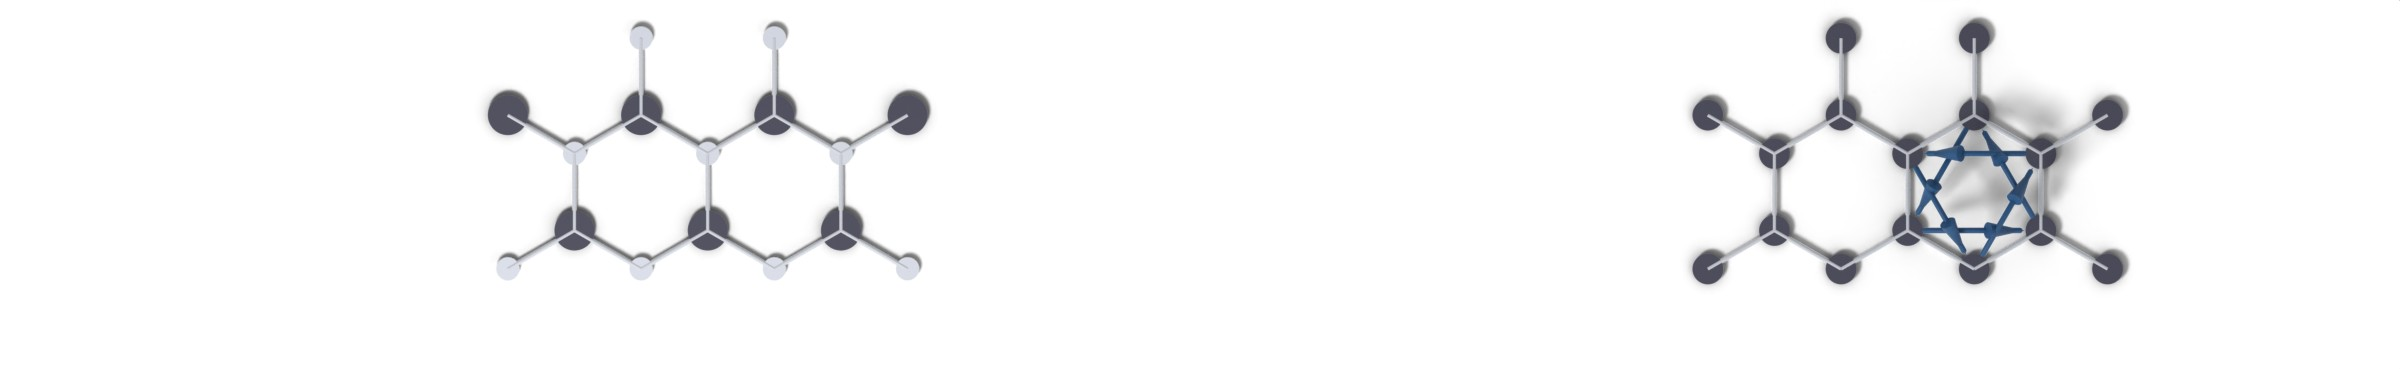
\includegraphics[width=\figw]{../blender/out/s03f05_masses_lat.jpg}};
    % written by build_figure.sh; the painted part of the image
\path (0.2000\figw,0.0329\figw) rectangle (0.8879\figw,0.1483\figw);

    %% written by figlib.py; x and y in units of the image width
\coordinate (lata) at (0.1795\figw,0.0769\figw);
\coordinate (latt2) at (0.8707\figw,0.0866\figw);
\coordinate (latb) at (0.6795\figw,0.0769\figw);

    \node[pnl, anchor=east, align=right] at (lata) {(a)\\\normalfont staggered\\\normalfont potential $\pm m$};
    \node[pnl, anchor=east, align=right] at (latb) {(b)\\\normalfont Haldane coupling\\\normalfont $t_2e^{\pm i\pi/2}$};
    \node[lbl, anchor=west, text=aqmaccent] at (latt2) {$t_2$};
    \draw[axarrow] (latrO) -- (latrx);
  \draw[axarrow] (latrO) -- (latry);
  \node[axlbl, anchor=north] at (latrx) {$x$};
  \node[axlbl, anchor=east] at (latry) {$y$};
\end{scope}
  \node[overlay, anchor=south west, inner sep=0pt] at (0,0)
    {
\includegraphics[width=\figw]{../blender/out/s03f05_masses_spec.jpg}};
  % written by build_figure.sh; the painted part of the image
\path (0.1367\figw,0.0013\figw) rectangle (0.9988\figw,0.1592\figw);

  %% written by figlib.py; x and y in units of the image width
\coordinate (aE) at (0.1392\figw,0.1514\figw);
\coordinate (ak0) at (0.1392\figw,0.0151\figw);
\coordinate (ak2pi) at (0.3608\figw,0.0151\figw);
\coordinate (akx) at (0.2500\figw,0.0151\figw);
\coordinate (bE) at (0.6392\figw,0.1514\figw);
\coordinate (bk0) at (0.6392\figw,0.0151\figw);
\coordinate (bk2pi) at (0.8608\figw,0.0151\figw);
\coordinate (bkx) at (0.7500\figw,0.0151\figw);

  \foreach \p in {a,b} {
    \node[lbl, anchor=south west] at (\p E) {$E$};
    \node[lbl, anchor=north] at (\p k0) {$0$};
    \node[lbl, anchor=north] at (\p k2pi) {$2\pi$};
    \node[lbl, anchor=north] at (\p kx) {$k_x$};
  }
  \aqmkey{(6.55cm,2.35cm)}{keydark}{top edge}{keylight}{bottom edge}
\end{tikzpicture}
\end{document}
